% Multi-candidate latent-label identifiability: a new knowable regime that removes the
% single-candidate calibration crutch (at the price of a different, CHECKABLE structural
% condition). Numbers from scripts/multicandidate_feasibility_probe.py
% (results/theory/feasibility_probe_results.json). \input from kbound.tex in §5.

The per-family boundaries above each pay a structural price (covariate shift, a known
drift radius, or known class-conditionals). This subsection enlarges the knowable region
along a different axis: instead of one candidate $f_a$, use several
($f_a^{(1)},\dots,f_a^{(M)}$, e.g.\ Tent, EATA, SAR) and identify the accuracy ordering on
the disagreement region from their \emph{joint} label-free agreements. By
Theorems~\ref{thm:disagree}--\ref{thm:disagree-mc} this ordering is exactly what fixes
$\sign\Delta$. The price becomes a \emph{checkable} condition rather than an untestable
premise.

\begin{definition}[Conditional error-independence on $D$]\label{def:cei}
On the disagreement region $D$ with latent label $Y$, candidates' correctness indicators
$\{\mathbf1[f_a^{(j)}(X){=}Y]\}_{j=1}^M$ are \emph{conditionally independent given $Y$}.
\end{definition}

\begin{theorem}[Multi-candidate ordering identifiability]\label{thm:multicand}
Let $Y\in\{0,1\}$ on $D$, $M\ge3$ candidates with accuracies $a_j=\Pr(f_a^{(j)}{=}Y\mid D)\neq\tfrac12$
and advantages $b_j=2a_j-1$. Under Definition~\ref{def:cei}, the pairwise agreement rates
$A_{ij}=\Pr(f_a^{(i)}{=}f_a^{(j)}\mid D)$ satisfy
\[
2A_{ij}-1 \;=\; b_i b_j \;=:\; c_{ij},
\]
so for any distinct $i,k,l$, $\;b_i^2=c_{ik}c_{il}/c_{kl}$, and the sign of $b_i$ is fixed
by an anchor (e.g.\ the majority of candidates exceeds chance). Hence every $a_j$ --- thus
the full ordering and every $\sign(a_i-a_j)$ --- is identified from label-free agreements
alone, with \emph{no} target labels and \emph{no} calibration-transfer assumption.
Combined with Theorems~\ref{thm:disagree}--\ref{thm:disagree-mc}, $\sign\Delta$ for any
candidate is label-free identifiable on $D$.
\end{theorem}
\emph{(Proof deferred to Appendix~\ref{app:proofs}.)}

\begin{proposition}[A sound checkable diagnostic, $M\ge4$]\label{prop:cei-test}
For $M\ge4$ the products $\{c_{ij}\}$ must factor as a rank-one form $c_{ij}=b_ib_j$;
this is overdetermined, e.g.\ $c_{12}c_{34}=c_{13}c_{24}=c_{14}c_{23}$. Define the
label-free residual $\tau=\max\{\cdot\}-\min\{\cdot\}$ of these products. Under
Definition~\ref{def:cei}, $\tau=0$; therefore $\tau>0$ \emph{certifies that conditional
error-independence is violated}. The test is sound one-sided (it never falsely rejects a
truly independent triple in the population limit) and is exactly the verifiability that
agreement-based accuracy heuristics (ATC, Agreement-on-the-Line, AETTA) leave implicit.
\end{proposition}
\emph{(Proof deferred to Appendix~\ref{app:proofs}.)}

\noindent\emph{Converse (honest, partial).} Definition~\ref{def:cei} is \emph{sufficient},
not necessary. Without a structural restriction the sign is genuinely unrecoverable:
given any agreement tensor one can correlate the candidates' errors to move
$\E[\delta\mid D]$ across zero while leaving all pairwise agreements fixed, instantiating
Theorem~\ref{thm:imp}. So the multi-candidate route \emph{trades} the single-candidate
calibration crutch for a \emph{checkable} independence condition --- it does not remove
structure altogether. Characterizing the \emph{weakest} (ideally testable) condition, and
its tight converse, is the open problem of Conjecture~\ref{conj:gen}.

\noindent\emph{Multiclass.} For $Y\in\{1,\dots,K\}$ the same conditional-independence
structure makes the per-candidate confusion matrices identifiable from second- and
third-order agreement tensors up to a global label permutation (Dawid--Skene; Anandkumar
et al.\ tensor decomposition), fixed by the same anchor; the accuracy ordering on $D$
follows. We use the binary case as the proved, validated core and cite the tensor
machinery for $K>2$.

\noindent\emph{Numerically validated}
(\texttt{multicandidate\_feasibility\_probe.py}; Fig.~\ref{fig:multicand}). Under
Definition~\ref{def:cei} the $M{=}3$ estimator recovers accuracies to max error $0.012$
and the ordering on $96\%$ of random draws; as error-correlation $\rho$ grows the
ordering degrades (the condition is the crux, as the theory says); and the $M{=}4$
diagnostic residual is $\approx\!0$ under independence and rises monotonically with
$\rho$ (Pearson $0.98$) --- a working, sound-one-sided check.

\begin{figure}[t]\centering
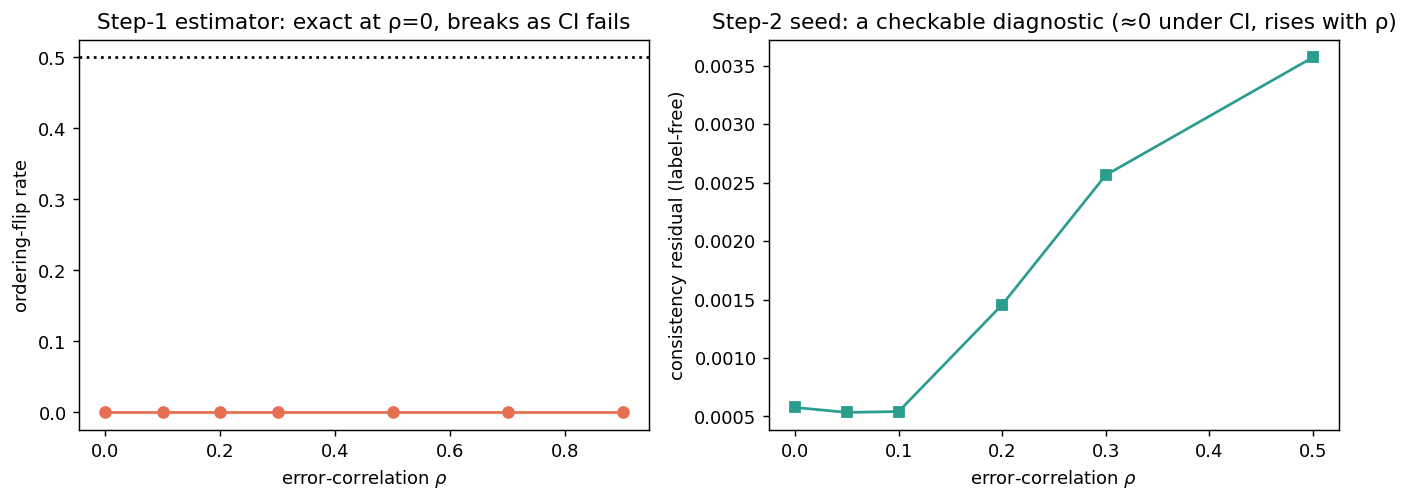
\includegraphics[width=0.92\textwidth]{figures/final/fig_feasibility.png}
\caption{Multi-candidate identifiability (Theorem~\ref{thm:multicand},
Proposition~\ref{prop:cei-test}). Left: the label-free ordering estimator is exact under
conditional error-independence and degrades as it fails. Right: the overdetermination
residual is a checkable diagnostic --- $\approx\!0$ under independence, rising with
error-correlation.}
\label{fig:multicand}
\end{figure}

\paragraph{Weight (honest).} The agreement estimator itself is classical---the rank-one accuracy-from-agreement method of Parisi et al.\ (2014) and Jaffe et al.\ (2015) under conditional independence; our contribution is its use as a label-free \emph{decision certificate} with the checkable overdetermination diagnostic (Proposition~\ref{prop:cei-test}), not the estimator. Unlike reactive risk monitors for TTA (Schirmer \& Jazbec, 2025), the certificate decides \emph{before} committing and carries an explicit abstain region. This \emph{enlarges} the knowable region beyond the
single-candidate certificate: where one candidate must abstain for want of calibration,
$M\ge3$ candidates can certify $\sign\Delta$ under a condition that is, crucially,
\emph{testable} (Proposition~\ref{prop:cei-test}) --- the guarantee that agreement-based
heuristics (ATC, AoL, AETTA) use empirically but never establish. It is not an
assumption-free result: it substitutes conditional error-independence (often violated by
co-trained models, which is exactly why the diagnostic matters) for the earlier crutches.
The assumption-free dichotomy --- the weakest checkable condition with a tight matching
converse --- remains open and is the stated frontier of this program
(Conjecture~\ref{conj:gen}).
